% ------------------------------------------------------------------
\documentclass[12 pt]{article} % A4 paper set by geometry package below
\pagenumbering{arabic}
\setlength{\parindent}{10 mm}
\setlength{\parskip}{12 pt}

% Nimbus Sans font should be reasonably legible
\usepackage{helvet}
\renewcommand{\familydefault}{\sfdefault}
\usepackage[T1]{fontenc}  % Without this \textsterling produces $

% Section header spacing
\usepackage{titlesec}
\titlespacing\section{0pt}{12pt plus 4pt minus 2pt}{0pt plus 2pt minus 2pt}
\titlespacing\subsection{0pt}{12pt plus 4pt minus 2pt}{0pt plus 2pt minus 2pt}
\titlespacing\subsubsection{0pt}{12pt plus 4pt minus 2pt}{0pt plus 2pt minus 2pt}

\usepackage{amsmath}
\usepackage{amssymb}
\usepackage{graphicx}
\usepackage{verbatim}    % For comment
\usepackage[shortlabels]{enumitem}
\usepackage[paper=a4paper, marginparwidth=0 cm, marginparsep=0 cm, top=2.5 cm, bottom=2.5 cm, left=3 cm, right=3 cm, includemp]{geometry}
\usepackage[pdftex, pdfstartview={FitH}, pdfnewwindow=true, colorlinks=true, citecolor=blue, filecolor=blue, linkcolor=blue, urlcolor=blue, pdfpagemode=UseNone]{hyperref}

% Put module code and last-modified date in footer
\usepackage{fancyhdr}
\pagestyle{fancy}
\fancyhf{}
\renewcommand{\headrulewidth}{0pt}
\cfoot{{\small \thisweek}\hfill \thepage\hfill {\small \moddate}}

% Hopefully address Canvas complaints about pdf tagging
%\usepackage[tagged]{accessibility}
% ------------------------------------------------------------------



% ------------------------------------------------------------------
\begin{document}
\newcommand{\thisweek}{MATH327 Extra (Cycle)}
\newcommand{\moddate}{Last modified 21 Mar.~2021}
\begin{center}
  {\Large \textbf{MATH327: Statistical Physics, Spring 2021}} \\[12 pt]
  {\Large \textbf{Extra practice \ --- \ Thermodynamic cycle}} \\[24 pt]
\end{center}

An ideal gas in a container can access two different thermal reservoirs: a hot reservoir with high temperature $T_H$ and a cold reservoir with low temperature $T_L < T_H$.
The system carries out the thermodynamic cycle illustrated by the $PV$~diagram below, where the processes $A \to B$ and $C \to D$ are adiabatic.
The five variables coloured red are given as inputs: The pressure $P_A$ at point $A$; The volume $V_A$ at points $A$ and $D$; The volume $V_B$ at points $B$ and $C$; The temperature $T_H$ at point $A$; The temperature $T_L$ at point $C$.

\begin{center}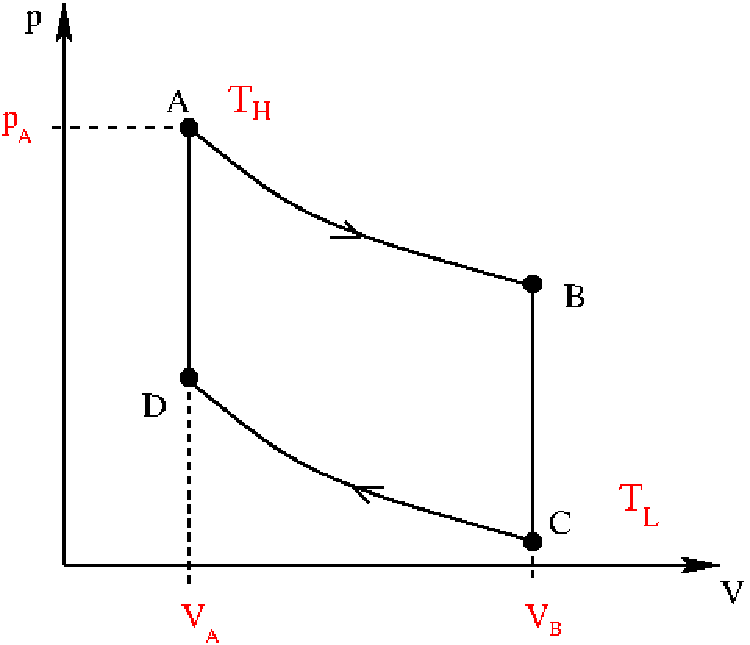
\includegraphics[width=0.6\textwidth]{figs/cycle.pdf}\end{center}

\begin{enumerate}[label={(\alph*)}]
  \item Describe the four stages of the cycle.
        What is kept fixed by each process?
        Is each process fast or slow, or is there not enough information to be sure?
  \item Calculate whatever variables $\left\{P, V, T\right\}$ are unknown at points $B$, $C$ and $D$.
  \item What are the highest temperature and the lowest temperature in the cycle?
  \item How much work is done by each stage of the cycle?
        In each case, if work is done, is it done by the system on its surroundings, or by the surroundings on the system?
  \item How much heat is exchanged in each stage of the cycle?
        In each case, if heat is exchanged, does it flow into or out of the system, and which thermal reservoir is involved?
  \item What is the efficiency of the cycle?
        How does this efficiency compare to the efficiency of the Carnot cycle?
\end{enumerate}

\end{document}
% ------------------------------------------------------------------
